% STATUS: ACTIVE -- gain-law form 2 (co-equal with powerlaw); WARNING body lags code (body=7b differential, code=7a algebraic motion_control_law_5state_expgain_alg.m)
% ======================================================
% Compile: xelatex 5state_expgain_hd.tex
% Path:    reference/eq17_analysis/derivation/5state_expgain_hd.tex
% Purpose: 5-state eq17 controller + closed-loop EKF with a SATURATING
%          EXPONENTIAL gain law
%              a_h(hbar) = a_o [ 1 - exp(-b phi(hbar)) ],   phi(hbar) = ln hbar,
%          replacing the power-law-in-(hbar-1) gain law of 5state_powerlaw_hd.tex.
%          Sub-state [a_h, b]: gain level + exponent constant.  The shape function
%          phi is isolated behind B[k] := b phi'(hbar_d[k]) so that changing phi
%          touches one definition only.
%          FULLY NON-DIMENSIONAL: every length is divided by the probe radius R,
%          so R survives only in three defining relations and never in the
%          derivation body.  Forces stay in pN.
%          State x = [ dh1, dh2, dh3, a_h, b ].
% ---- NOTES (deliberately kept out of the PDF; they belong to the implementation) ----
%  * y2 is NOT an independent physical measurement.  It is the gain read back out of
%    the variance of the same dh_m stream that feeds y1:
%        u[k] = (dh_r^2[k] - C_n sig_nh^2) / (C_dpmr (4kBT/R)),  E u[k] = a_h[k-d]
%    Two consequences the body does not model, both known and accepted for now:
%      (i)  u is colored.  dh_r has rho(1) ~ 0.85, so by Wick rho_u(1) ~ 0.72.  The
%           reported a_hm is an EWMA of u, so its pole is NOT 1-a_cov; the true pole
%           needs Yule-Walker (see compute_y2_ar1_phi in build_eq17_6state_constants).
%      (ii) n_a and n_h are correlated (same data used twice), so R = diag(R1,R2)
%           is an approximation.
%    A candidate fix is to feed the whitened increment y2 = a_hm[k]-(1-a_cov)a_hm[k-1]
%    = a_cov*u[k], which cancels the EWMA pole and the ~19-step group delay; its
%    acceptance test is invariance of the result to a_cov.  NOT adopted in the body.
%  * b's channel through y2 is very weak: |H(2,5)|/sqrt(R2) ~ 0.0075 per sample at
%    hbar=2.  b is identified mainly through the F_e(4,5) dynamic coupling, not y2.
%    Consistent with the 2026-07-27 experiments (switching y2 off costs only 0.8%).
%  * C_dpmr, C_n are the full-a_pd closed forms implemented in
%    build_eq17_6state_constants (3.1610, 1.1093 at lc=0.7, a_pd=0.05).  The a_pd->0
%    simplification 2+1/(1-lc^2), 2/(1+lc) is stale and biases a_hm by -20%.
%  * F_e row 4: the exact multiplier of e_ah and e_b is Dhbar_d + (1-lc)dh3 + eps_h,
%    with F_dh*e_ah entering separately as the +a'_h F_dh term.  Only eps_h is dropped
%    (zero mean, unknown to the filter).  (1-lc)dh3 is the same order as Dhbar_d and
%    known as (1-lc)dh3_hat; dropping it would zero F_e(4,5) at every trajectory
%    turning point (Dhbar_d = 0).
%  * The innovation line a'_h - a'_h_hat = -B_hat*e_ah + (a'_h/b)*e_b is an exact
%    identity (mixed evaluation points), not an approximation.  An implementation
%    must use a'_h_hat/b_hat, which costs -phi'*e_ah*e_b, second order.
%  * The dropped grad*B_hat term in dy2/da_h is FIRST order in e_ah (not second):
%    the residual is grad*phi'*b*e_ah, relative size grad*B_hat ~ 0.4% at hbar=2
%    (1 Hz / 2.5 um).  It is dropped because dy2/da_h's leading term is O(1); the
%    same O(grad) term is KEPT in dy2/db because there it is the whole entry.
%  * B[k] is evaluated at the commanded hbar_d while a_h is at the true point.  This
%    mixing is deliberate (B must be computable from the command alone); the error is
%    O(phi'' * dh3), relative dh3/hbar ~ 0.5%.
%  * Evaluate at the current estimate in code: F_e and H entries (B_hat, a'_h_hat,
%    b_hat) AND the Q/R entries (Q33, Q44, R2 all carry a_h, a'_h, written here as
%    true values because they are true statistics).
%  * All lengths, sigma_nh included, are already divided by R.  Feeding a sensor
%    variance in um^2 would be wrong by R^2 = 5.06.
%  * Q33: fluctuation-dissipation and the gain must use the SAME local drag
%    gamma(hbar) = gamma_N c(hbar); c cancels and Q33 follows a_h[k].
%  * R2's d*Q44 term only covers part of the back-off residual.  The exact residual
%    is a'_h*(dh3[k]-dh1[k]), which also carries (1-lc)*sum(dh3) and F_dh*sum(e_ah);
%    at lc=0.7 the doc term is low by (2-lc)=1.3x and misses the sig_nh channel.
%    It is <6e-4 of R2, so numerically irrelevant.  Note that dh1 and dh3 are both
%    states, so the residual could instead be moved into H exactly:
%    ADD H(2,1) = -a'_h_hat and H(2,3) = +a'_h_hat (both entries are currently zero),
%    and then R2 needs no delay term at all.
%  * Known Q-R cross-correlation: n_h appears both in R1 and inside eps_h's
%    (1-lc)n_h, so E[q3*r1] = -(1-lc)sig_nh^2 != 0 (corr ~0.27 at hbar=2).  This is
%    the project's existing Path C / Eq.19-form trade-off, not introduced here.
%  * Verified by four independent agents (algebraic re-derivation + sympy).  One of
%    them also checked, and rejected, evaluating B at the estimated height
%    hhat = hbar_d - dh3_hat: the partial at fixed a_h is +a'_h/hbar (NOT -a''_h --
%    a'' is the total derivative along the curve and double-counts the a_h path
%    already carried by -B_hat*e_ah).  It buys only 1.41x (0.483% -> 0.343%, both
%    zero-mean; the Jensen bias of using hbar_d is 0.0023%) while a'_h's own model
%    truncation against the true c_perp is 2.43% RMS -- 5-7x larger.  Reverted.
% ---- BUILD STATUS: COMPLETE.  Stages 1-6: motion error / gain model / shape
%      acceptance (2b) / true state eq / output eq + H / estimator + error dynamics
%      + F_e / Q,R.  y2 is the direct (un-whitened) gain readout; F_e row 4
%      multiplier is Dhbar_d + (1-lc)dh3_hat; hat usage: true values in the physical
%      equations, estimates in H / F_e. ----
%  * Stage 2b defines b_eff (the exponent the true curve demands at each height) and
%    turns sup|b_eff - 1| into the acceptance test for the SHAPE, and into the only
%    defensible source for sqrt(P55[0]).  Numbers are from an offline sweep of the
%    exact correction polynomials (0.0942 perp / 0.778 para whole-domain, 0.0816 /
%    0.0342 for hbar >= 2).  REPRODUCE / RE-RUN AFTER ANY SHAPE CHANGE:
%       test_script/integration/verify_shape_exponent_bound.m   (tracked, not temp_*)
%    It prints this table, the anchor values at both ends, the coherent-vs-diffusive
%    Q55 comparison, the A^2/hbar_0^2 seed rule, and a PASS/TIGHT/FAIL verdict of
%    each shipped prior against its own bound.
%    It also records WHY the fix for a varying b is a new shape and not Q55 > 0: the
%    variation is commanded (prop. to Dhbar_d), hence coherent (~N), while a random
%    walk diffuses (~sqrt N) and falls 5x short over the canonical descent.
%  * Pf_b_std = 0.10 in the controller currently clears the perp bound by only 1.06x.
%    If the shape is re-derived, re-run the sweep and re-set the prior from it.
% ======================================================
\documentclass[11pt,a4paper,fontset=none]{ctexart}

\usepackage[fleqn]{amsmath}
\usepackage{amssymb,bm}
\usepackage{empheq}
\setlength{\mathindent}{0pt}
\usepackage{geometry}
\geometry{margin=2.0cm}
\usepackage{enumitem}
\usepackage{array,booktabs}
\usepackage{titlesec}
\usepackage{graphicx}

\setlength{\parindent}{0pt}
\setlength{\parskip}{0.80em}
\linespread{1.08}
\setlength{\abovedisplayskip}{10pt}
\setlength{\belowdisplayskip}{10pt}
\setlength{\abovedisplayshortskip}{5pt}
\setlength{\belowdisplayshortskip}{5pt}

% --- Shortcuts (non-dimensional h-notation, exponential gain) ---
\newcommand{\lc}{\lambda_c}
\newcommand{\hbn}{\bar h}
\newcommand{\hb}{\bar h_d}
\newcommand{\dhb}{\delta\bar h}
\newcommand{\Dhb}{\Delta\bar h_d}
\newcommand{\Ghb}{\nabla_{\!d}\bar h_d}
\newcommand{\Fdh}{F_{dh}}
\newcommand{\ao}{a_{o}}
\newcommand{\aph}{a_h'}
\newcommand{\aphat}{\hat a_h'}
\newcommand{\eah}{e_{a_h}}
\newcommand{\eb}{e_{b}}
\newcommand{\hd}[1]{\par\smallskip\noindent\underline{\textbf{#1}}\par\nobreak\vspace{0.1ex}}

\begin{document}

\hd{Equation of motion}
\[ \hbn[k+1] = \hbn[k] + a_h[k]\{f_{dh}[k] + f_T[k]\} + \dhb_D[k], \]

\vfill
\hd{Motion error}
\[ \dhb[k+1] = \dhb[k] + \Dhb[k] - a_h[k]\{f_{dh}[k] + f_T[k]\} - \dhb_D[k], \]
\[ \dhb[k] = \hb[k] - \hbn[k], \qquad \Dhb[k] = \hb[k{+}1] - \hb[k] \]

\vfill
\hd{Measurement} (\textit{d}-step delay)
\[ \dhb_m[k] = \dhb[k-d] + n_h[k], \qquad\qquad
   \textbf{Control objective}: \;\; \dhb[k+1] = \lc\,\dhb[k], \quad 0 \le \lc < 1 \]

\vfill
\textit{Ideal control effort (no measurement delay)}, and the resulting motion error:
\[ \bar f_{dh}[k] = a_h^{-1}[k]\{\Dhb[k] + (1-\lc)\,\bm{\dhb[k]} - \dhb_D[k]\} \]
\[ \dhb[k+1] = \dhb[k] + \Dhb[k] - a_h[k]\{\bar f_{dh}[k] + f_T[k]\} - \dhb_D[k] = \lc \cdot \dhb[k] - a_h[k] f_T[k] \]

\vfill
\textit{d-step measurement delay}:
\[ \bm{\dhb[k]} = \dhb[k-d] + \sum_{i=1}^{d}\Dhb[k-i] - \sum_{i=1}^{d} a_h[k-i]\{f_{dh}[k-i] + f_T[k-i]\} - \sum_{i=1}^{d}\dhb_D[k-i] \]

\vfill
\textit{Ideal control effort (with d-step measurement delay)}:
\[
\begin{aligned}
\bar{\bar f}_{dh}[k] = a_h^{-1}[k]\Big\{
& \Dhb[k] - \dhb_D[k]
+ (1-\lc)\textstyle\sum_{i=1}^{d}\Big[\Dhb[k-i] - \dhb_D[k-i]\Big] \\
& + (1-\lc)\Big[\dhb[k-d] - \textstyle\sum_{i=1}^{d} a_h[k-i] f_{dh}[k-i]\Big]
\Big\}
\end{aligned}
\]
\[
\dhb[k+1] = \lc \cdot \dhb[k] - \Big\{ a_h[k] f_T[k] + (1-\lc)\textstyle\sum_{i=1}^{d} a_h[k-i] f_T[k-i] \Big\}
\]

\vfill
\hd{Implementable control effort} \;{\small (disturbance not estimated)}
\begin{empheq}[box=\fbox]{equation*}
f_{dh}[k] = \hat a_h^{-1}[k]\Big\{ \Dhb[k] + (1-\lc)\Big[\textstyle\sum_{i=1}^{d}\Dhb[k-i]
+ \dhb_m[k] - \textstyle\sum_{i=1}^{d}\hat a_h[k-i] f_{dh}[k-i]\Big] \Big\}
\end{empheq}

\newpage

\hd{Motion error}
\[ \dhb[k+1] = \lc \cdot \dhb[k] - a_h[k]\big[ f_{dh}[k] - \bar{\bar f}_{dh}[k] \big]
   - \Big\{ a_h[k] f_T[k] + (1-\lc)\textstyle\sum_{i=1}^{d} a_h[k-i] f_T[k-i] \Big\} \]

\[
\begin{aligned}
a_h[k]\, f_{dh}[k] - a_h[k]\,\bar{\bar f}_{dh}[k] ={}& \eah[k]\, f_{dh}[k] + (1-\lc) n_h[k] \\
&+ (1-\lc)\textstyle\sum_{i=1}^{d}\big(a_h[k-i] - \hat a_h[k-i]\big) f_{dh}[k-i] \\
&+ \dhb_D[k] + (1-\lc)\textstyle\sum_{i=1}^{d}\dhb_D[k-i]
\end{aligned}
\]

\textit{Gain-error back-step}:
\[ a_h[k-i] - \hat a_h[k-i] \approx \eah[k] - \big(\hb[k]-\hb[k-i]\big)\,\big(\aph[k]-\hat a_h'[k]\big) \approx \eah[k] \]
\[
\begin{aligned}
a_h[k]\, f_{dh}[k] - a_h[k]\,\bar{\bar f}_{dh}[k] \approx{}&
\eah[k]\,\underbrace{\Big\{ f_{dh}[k] + (1-\lc)\textstyle\sum_{i=1}^{d} f_{dh}[k-i] \Big\}}_{\Fdh[k]} \\
&+ \dhb_D[k] + (1-\lc)\textstyle\sum_{i=1}^{d}\dhb_D[k-i] + (1-\lc) n_h[k]
\end{aligned}
\]

\begin{empheq}[box=\fbox]{align*}
\dhb[k+1] ={}& \lc \cdot \dhb[k] - \Fdh[k]\cdot \eah[k]
 - \dhb_D[k] - (1-\lc)\textstyle\sum_{i=1}^{d}\dhb_D[k-i] - \varepsilon_h[k] \\
\varepsilon_h[k] :={}& a_h[k] f_T[k] + (1-\lc)\textstyle\sum_{i=1}^{d} a_h[k-i] f_T[k-i] + (1-\lc)\,n_h[k]
\end{empheq}

% ======================================================
% Stage 2 --- Gain model
% ======================================================

\hd{Gain model} \;{\small ($\ao = \Delta t/(\gamma_N R)$ = far-field gain, $\hb = h_d/R$; $a_h$ has units $1/$pN)}

\[ a_h(\hbn) = \ao\big[\,1 - e^{-b\,\varphi(\hbn)}\,\big],
   \qquad \varphi(1) = 0,\quad \varphi(\hbn\to\infty) = \infty,\quad \varphi' > 0 \]

\[ \aph(\hbn) := \frac{d a_h}{d\hbn}
   = \varphi'(\hbn)\,b\,\ao\,e^{-b\varphi(\hbn)}
   = \varphi'(\hbn)\,b\,\big[\ao - a_h(\hbn)\big] \]

\[ B[k] := b\,\varphi'(\hb[k])
   \qquad\Longrightarrow\qquad
   \aph[k] = B[k]\,\big[\ao - a_h[k]\big]
   \qquad {\small\text{($b$ is a state, $B[k]$ is not)}} \]

\hd{Shape function}
\[ \varphi(\hbn) = \ln\hbn
   \qquad\Longrightarrow\qquad
   \varphi'(\hbn) = \frac{1}{\hbn},
   \qquad B[k] = \frac{b}{\hb[k]},
   \qquad a_h(\hbn) = \ao\big[\,1 - \hbn^{-b}\,\big] \]

\begin{empheq}[box=\fbox]{align*}
a_h(\hbn) &= \ao\big[\,1 - e^{-b\varphi(\hbn)}\,\big], &
\aph[k] &= B[k]\,\big[\ao - a_h[k]\big], &
b[k{+}1] &= b[k], \\
\varphi(\hbn) &= \ln\hbn, &
B[k] &= b\,\varphi'(\hb[k]) = b/\hb[k]. &&
\end{empheq}

% ======================================================
% Stage 2b --- Shape acceptance: what pins b = 1, and how wide its prior must be
% ======================================================

\hd{Local exponent demanded by the true curve}

The gain law asserts that the normalised gain deficit is a pure exponential in $\varphi$:
\[ \Psi(\hbn) := 1 - \frac{a_h(\hbn)}{\ao} = e^{-b\varphi(\hbn)},
   \qquad\text{true value}\quad
   \Psi_{\rm true}(\hbn) = 1 - \frac{1}{c(\hbn)} = \frac{c-1}{c} \]

so $b$ is \emph{by construction} a slope in $(\ln\Psi,\varphi)$ coordinates. Reading that
slope off the true curve gives the exponent the truth demands at each height:
\[ b = -\frac{d\ln\Psi}{d\varphi}
   \qquad\Longrightarrow\qquad
   b_{\rm eff}(\hbn) := -\frac{1}{\varphi'(\hbn)}\,\frac{d}{d\hbn}\ln\frac{c-1}{c}
   = -\,\frac{\hbn\,c'(\hbn)}{c(\hbn)\,\big[c(\hbn)-1\big]} \]

Were the shape exact, $b_{\rm eff}$ would be constant. \textbf{Its variation is the model
error}, and it is the only quantity that can set the prior on $b$: $b$ is a parameter of an
approximate shape, not a physical constant, so ``how wrong is $\hat b[0]=1$'' has no meaning
beyond ``how far does $b_{\rm eff}$ stray from $1$ over the reachable domain''.

\hd{Two limits pin $b = 1$} \;{\small (both read off the published asymptotics; $c$ itself is never needed at run time)}
\[
\begin{aligned}
\hbn\to1:&\quad c \to \tfrac{K}{\hbn-1} \;\Rightarrow\; \ln\Psi \simeq -\tfrac{\hbn-1}{K},
  \;\; \varphi \simeq \hbn-1 &&\Rightarrow\quad b_{\rm eff} \to 1/K \\
\hbn\to\infty:&\quad c-1 = A\hbn^{-1}+A^2\hbn^{-2}+\dots \;\Rightarrow\; \Psi = A\hbn^{-1}+O(\hbn^{-3}),
  \;\; \ln\Psi = \ln A - \varphi &&\Rightarrow\quad b_{\rm eff} \to 1
\end{aligned}
\]

The far-field anchor is coefficient-free ($A$ is additive in $\ln\Psi$, so it drops out of the
slope), and the $O(\hbn^{-2})$ terms cancel identically in $\Psi=(c-1)/c$ --- which is why the
exponential shape is \emph{more} accurate far from the wall than the power law
($b_{\rm eff}=0.9983$ vs $p_{\rm eff}=1.0042$ at $\hbn=22.2$). The near-wall anchor is
\emph{weaker} than the power law's: it returns $1/K$, so it pins $b=1$ only because Brenner
lubrication carries unit coefficient $K=1$, whereas the power law's near-wall anchor gives $1$
for any $K$.

\hd{Acceptance criterion} \;{\small (evaluated offline once on the exact correction polynomials; the controller carries only the resulting number)}

\begin{center}
{\small
\begin{tabular}{llcccc}
\toprule
 & & \multicolumn{2}{c}{$\perp$ \; ($c_\perp$)} & \multicolumn{2}{c}{$\parallel$ \; ($c_\parallel$)} \\
\cmidrule(lr){3-4}\cmidrule(lr){5-6}
shape & exponent & all $\hbn$ & $\hbn\ge2$ & all $\hbn$ & $\hbn\ge2$ \\
\midrule
power law \; $c-1 = K(\hbn-1)^{-p}$ & $p$ & 0.034 & 0.024 & 0.994 & 0.283 \\
exponential \; $\Psi = \hbn^{-b}$   & $b$ & 0.094 & 0.082 & 0.778 & \textbf{0.034} \\
\bottomrule
\end{tabular}}
\end{center}
{\small Tabulated: $\sup|\text{exponent}-1|$. The exponential shape trades $\perp$ accuracy
($2.8$--$3.4\times$ worse) for $\parallel$ viability ($8.3\times$ better over the working range),
which is what lets one gain law serve all three axes; the power law has no near-wall anchor for
$\parallel$ at all, since $c_\parallel$ stays finite at contact.}

Since $b$ is modelled as constant, $P_{55}[0]$ is the entire budget the filter may spend on it
($Q_{55}=0$ and $\mathbf F_e$ row 5 $=[0\,0\,0\,0\,1]$ give
$\mathbb E[(\hat b_\infty-\hat b_0)^2] = P_{55}[0]-P_{55}[\infty]$). The shape is therefore
acceptable exactly when that budget covers its own mismatch:

\begin{empheq}[box=\fbox]{equation*}
\sup_{\hbn}\,\big|\,b_{\rm eff}(\hbn) - 1\,\big| \;\;\lesssim\;\; \sqrt{P_{55}[0]}
\qquad\Longleftrightarrow\qquad
Q_{55} = 0 \;\text{is honest}
\end{empheq}

{\small \textbf{Current status.} $\sqrt{P_{55}[0]} = 0.10$ against $0.0942$ for $\perp$: the
criterion is met with a factor $1.06$, i.e.\ no margin. (The power law on $\perp$ sat at
$0.035$ against $0.034$ --- the same tightness.) A shape whose exponent varied by, say,
$0.01$ would let the prior shrink by an order of magnitude and turn $b$ from a nuisance
parameter into an identified one.}

\hd{Why a non-zero $Q_{55}$ is the wrong repair}

If $b_{\rm eff}$ varies with height, the true exponent moves as
\[ b_{\rm true}[k{+}1] - b_{\rm true}[k] = \frac{db_{\rm eff}}{d\hbn}\,\Dhb[k] \]
which is \emph{deterministic and commanded}: $\Dhb$ is the trajectory increment, known exactly
and noise-free. Such a term belongs in the prediction as a feedforward on row 5, not in $Q$.
Modelling it as a random walk, $Q_{55}[k] = \kappa_b^2\,\Dhb^2[k]$ with
$\kappa_b := \sup|db_{\rm eff}/d\hbn| = 0.032$ ($\perp$, $\hbn\ge2$), does keep the correct
trajectory gating --- $Q_{55}=0$ while holding, since $b_{\rm true}$ does not move when the
probe does not --- but it diffuses as $\sqrt N$ where the true drift accumulates as $N$: over
the canonical descent $\hbn: 22.2\to2$ in $N=1600$ steps it supplies
$\kappa_b\sqrt N\,\Dhb = 0.016$, while $b_{\rm eff}$ actually travels
$0.9983\to0.9184 = 0.080$ --- short by $5\times$ even with $\kappa_b$ taken as a supremum.
Inflating $\kappa_b$ only contaminates the hold phases without restoring the shape. The exact
feedforward needs $db_{\rm eff}/d\hbn$, i.e.\ $c$ itself, which this gain law exists to avoid;
estimating it instead adds a state and reopens the Taylor-ladder regress the two-parameter law
was introduced to close. The criterion above is therefore stated on the shape, never on $Q$.

% ======================================================
% Stage 3 --- True state equation
% ======================================================

\hd{State} \;{\small ($\mathbf y$ carries $\dhb[k-d]$; $a_h$ and $b$ are unknown)}
\[ \dhb_j[k] := \dhb[k-d+j-1], \quad j = 1,\dots,d{+}1;
   \qquad \mathbf x[k] = \big[\, \dhb_1,\ \dhb_2,\ \dhb_3,\ a_h,\ b \,\big]^\top[k] \quad (d = 2) \]

\hd{Tracking error} \;{\small (boxed motion error, $\dhb_D \equiv 0$ hereafter)}
\[ \dhb_3[k+1] = \lc\,\dhb_3[k] - \Fdh[k]\,\eah[k] - \varepsilon_h[k] \]

\hd{Gain recursion} \;{\small (the gain is evaluated at the true point, which trails the command by $\dhb_3$)}
\[ \hbn[k] = \hb[k] - \dhb_3[k] \]
\[
\begin{aligned}
a_h[k]   &= a_h(\hb[k]) - \aph[k]\,\dhb_3[k] \\
a_h[k+1] &= a_h(\hb[k{+}1]) - \aph[k]\,\dhb_3[k{+}1]
          = a_h(\hb[k]) + \aph[k]\,\Dhb[k] - \aph[k]\,\dhb_3[k{+}1]
\end{aligned}
\]

Subtracting,
\[ a_h[k+1] = a_h[k] + \aph[k]\Big\{ \underbrace{\Dhb[k] - \big(\dhb_3[k{+}1] - \dhb_3[k]\big)}_{\text{step taken by the true position}} \Big\} \]

and substituting $\dhb_3[k{+}1]$,
\[ a_h[k+1] = a_h[k] + \aph[k]\Big\{ \Dhb[k] + (1-\lc)\,\dhb_3[k] + \Fdh[k]\,\eah[k] + \varepsilon_h[k] \Big\} \]

\hd{True state equation}
\begin{empheq}[box=\fbox]{align*}
\dhb_1[k+1] &= \dhb_2[k] \\
\dhb_2[k+1] &= \dhb_3[k] \\
\dhb_3[k+1] &= \lc\,\dhb_3[k] - \Fdh[k]\,\eah[k] - \varepsilon_h[k] \\
a_h[k+1]    &= a_h[k] + \aph[k]\big\{ \Dhb[k] + (1-\lc)\,\dhb_3[k] + \Fdh[k]\,\eah[k] + \varepsilon_h[k] \big\} \\
b[k+1]      &= b[k], \qquad\qquad \aph[k] = B[k]\big[\ao - a_h[k]\big]
\end{empheq}


% ======================================================
% Stage 4 --- Output equation
% ======================================================

\hd{Measurement} \;{\small (every length, $\sigma_{n_h}$ included, is already normalized by $R$)}
\[ \Ghb[k] := \hb[k] - \hb[k-d] \]
\[ y_1[k] = \dhb_m[k] = \dhb_1[k] + \underbrace{n_h[k]}_{r_1[k]} \]

\[ y_2[k] = a_{hm}[k] = a_h[k-d] + \underbrace{n_a[k]}_{r_2[k]} \]

\hd{Delay back-off}
\[ a_h[k-d] = a_h[k] - \aph[k]\,\Ghb[k]
   \qquad\Longrightarrow\qquad
   y_2[k] = a_h[k] - \aph[k]\,\Ghb[k] + n_a[k] \]

\hd{Linearization} \;{\small (Jacobian at the estimate; partials at fixed $a_h$, since $a_h$ and $b$ are independent states)}
\[ \frac{\partial y_2}{\partial a_h} = 1 + \Ghb[k]\,\hat B[k] \;\longrightarrow\; 1,
   \qquad
   \frac{\partial y_2}{\partial b} = -\,\Ghb[k]\,\frac{\aphat[k]}{\hat b} \]

\hd{Output equation} \;{\small ($\mathbf H$ is the Jacobian; the second row is nonlinear in $\mathbf x$, so $\mathbf H\mathbf x$ is its linearization, not an identity)}
\begin{empheq}[box=\fbox]{equation*}
\mathbf y[k] = \mathbf H[k]\,\mathbf x[k] + \mathbf r[k], \qquad
\mathbf H[k] = \begin{bmatrix}
1 & 0 & 0 & 0 & 0 \\[0.4ex]
0 & 0 & 0 & 1 & -\,\Ghb[k]\,\aphat[k]/\hat b
\end{bmatrix}, \qquad
\mathbf r[k] = \begin{bmatrix} n_h[k] \\[0.4ex] n_a[k] \end{bmatrix}
\end{empheq}


% ======================================================
% Stage 5 --- Estimator, error dynamics, F_e
% ======================================================

\hd{Estimation error}
\[ e_{\dhb_j} = \dhb_j - \delta\hat{\bar h}_j \;(j=1,2,3), \qquad
   \eah = a_h - \hat a_h, \qquad \eb = b - \hat b, \qquad
   \mathbf e = \big[\, e_{\dhb_1},\ e_{\dhb_2},\ e_{\dhb_3},\ \eah,\ \eb \,\big]^\top \]

\hd{Innovation} \;{\small ($\aphat = \hat B[k][\ao - \hat a_h]$, $\hat B[k] = \hat b\,\varphi'(\hb[k])$; the second line mixes evaluation points, which is what makes it exact)}
\[ e_{y_1} = y_1 - \delta\hat{\bar h}_1 = e_{\dhb_1} + n_h \]
\[ \aph - \hat a_h' = \varphi'(\hb)\big\{ b\,[\ao - a_h] - \hat b\,[\ao - \hat a_h] \big\}
   = -\,\hat B[k]\,\eah + \frac{\aph[k]}{b}\,\eb \]
\[
\begin{aligned}
e_{y_2} &= y_2 - \big(\hat a_h - \aphat\,\Ghb\big)
 = \big(1 + \Ghb\,\hat B[k]\big)\eah - \Ghb\,\frac{\aphat[k]}{\hat b}\,\eb + n_a \\
 &\longrightarrow\; \eah - \Ghb\,\frac{\aphat[k]}{\hat b}\,\eb + n_a
\end{aligned}
\]

\hd{Estimator} \;{\small ($\hat a_h$ swept by the step the estimator knows)}
\[
\begin{aligned}
\delta\hat{\bar h}_1[k+1] &= \delta\hat{\bar h}_2 + \ell_{11}e_{y_1} + \ell_{12}e_{y_2} \\
\delta\hat{\bar h}_2[k+1] &= \delta\hat{\bar h}_3 + \ell_{21}e_{y_1} + \ell_{22}e_{y_2} \\
\delta\hat{\bar h}_3[k+1] &= \lc\,\delta\hat{\bar h}_3 + \ell_{31}e_{y_1} + \ell_{32}e_{y_2} \\
\hat a_h[k+1] &= \hat a_h + \hat a_h'\big\{\Dhb + (1-\lc)\,\delta\hat{\bar h}_3\big\} + \ell_{41}e_{y_1} + \ell_{42}e_{y_2} \\
\hat b[k+1] &= \hat b + \ell_{51}e_{y_1} + \ell_{52}e_{y_2}
\end{aligned}
\]

\hd{Error dynamics} \;{\small (True $-$ Estimator; coefficients at the estimate)}
\[ {\small
\begin{aligned}
e_{\dhb_1}[k+1] &= e_{\dhb_2} - \ell_{11}e_{y_1} - \ell_{12}e_{y_2} \\
e_{\dhb_2}[k+1] &= e_{\dhb_3} - \ell_{21}e_{y_1} - \ell_{22}e_{y_2} \\
e_{\dhb_3}[k+1] &= \lc\,e_{\dhb_3} - \Fdh\,\eah + \underbrace{(-\varepsilon_h)}_{q_3} - \ell_{31}e_{y_1} - \ell_{32}e_{y_2} \\
\eah[k+1] &= \Big(1 - \big[\Dhb + (1{-}\lc)\delta\hat{\bar h}_3\big]\hat B + \aphat\Fdh\Big)\eah
             + (1{-}\lc)\aphat\,e_{\dhb_3}
             + \big[\Dhb + (1{-}\lc)\delta\hat{\bar h}_3\big]\tfrac{\aphat}{\hat b}\,\eb \\
          &\quad + \underbrace{\aph\varepsilon_h}_{q_4} - \ell_{41}e_{y_1} - \ell_{42}e_{y_2} \\
\eb[k+1] &= \eb - \ell_{51}e_{y_1} - \ell_{52}e_{y_2}
\end{aligned}}
\]

\hd{Error state equation} \;{\small ($\mathbf q = [\,0,\,0,\,q_3,\,q_4,\,0\,]^\top$, $q_3 = -\varepsilon_h$, $q_4 = \aph[k]\,\varepsilon_h = -\aph[k]\,q_3$; entries evaluated at the current estimate)}
\begin{empheq}[box=\fbox]{align*}
\mathbf e[k+1] &= \mathbf F_e[k]\,\mathbf e[k] - \mathbf L[k]\,\mathbf H[k]\,\mathbf e[k] + \mathbf q[k] \\[0.6ex]
\mathbf F_e[k] &= {\small
\begin{bmatrix}
0 & 1 & 0 & 0 & 0 \\
0 & 0 & 1 & 0 & 0 \\
0 & 0 & \lc & -\Fdh & 0 \\
0 & 0 & (1{-}\lc)\aphat & 1 - \big[\Dhb + (1{-}\lc)\delta\hat{\bar h}_3\big]\hat B + \aphat\Fdh & \big[\Dhb + (1{-}\lc)\delta\hat{\bar h}_3\big]\aphat/\hat b \\
0 & 0 & 0 & 0 & 1
\end{bmatrix}}
\end{empheq}

% ======================================================
% Stage 6 --- Q and R
% ======================================================

\hd{Process noise $Q$} \;{\small (only the current white thermal step enters $Q$: the past thermal steps in $\varepsilon_h$ are cross-step correlated, and $n_h$ already sits in $R_1$)}
\[ q_3 = -\,a_h[k]\,f_T[k], \qquad q_4 = \aph[k]\,a_h[k]\,f_T[k] = -\,\aph[k]\,q_3 \]
\[ \gamma(\hbn) = \gamma_N\,c(\hbn), \qquad
   \sigma_{f_T}^2 = \frac{4k_BT\,\gamma(\hbn)}{\Delta t}, \qquad
   a_h = \frac{\Delta t}{\gamma(\hbn)\,R} \]
\[ \mathrm{Var}\big(a_h f_T\big) = a_h^2\,\sigma_{f_T}^2 = \frac{4k_BT}{R}\,a_h[k] \]

\begin{empheq}[box=\fbox]{align*}
Q_{33}[k] &= \frac{4k_BT}{R}\,a_h[k], &
Q_{34}[k] = Q_{43}[k] &= -\,\aph[k]\,Q_{33}[k], \\
Q_{44}[k] &= \aph^2[k]\,Q_{33}[k], &
Q_{55} &= 0 \quad (b \text{ constant});
\end{empheq}
{\small All other entries vanish; the gain block is rank one, since $q_4 = -\aph[k]\,q_3$.}
\newpage

\hd{Measurement noise $R = \mathrm{diag}(R_1,R_2)$} \;{\small ($a_{cov}$ = EWMA coefficient, $\mathrm{IF}_{var}$ = MA($d$) inflation factor of $\hat\sigma^2_{\dhb_r}$)}
\[ R_1 = \sigma_{n_h}^2 \]

\[ \sigma^2_{\dhb_r}[k] = C_{dpmr}\,\frac{4k_BT}{R}\,a_h[k] + C_n\,\sigma_{n_h}^2
   = C_{dpmr}\,\frac{4k_BT}{R}\,\big(a_h[k] + \xi\big),
   \qquad \xi := \frac{C_n}{C_{dpmr}}\,\frac{\sigma_{n_h}^2}{4k_BT/R} \]
\[ a_{hm}[k] = \frac{\hat\sigma^2_{\dhb_r}[k] - C_n\,\sigma_{n_h}^2}{C_{dpmr}\,(4k_BT/R)} \]

\[ \mathrm{Var}\big(\hat\sigma^2_{\dhb_r}\big) = K_{var}\,\mathrm{IF}_{var}\,\big(\sigma^2_{\dhb_r}\big)^2,
   \qquad K_{var} = \frac{2a_{cov}}{2-a_{cov}} \]

\begin{empheq}[box=\fbox]{equation*}
R_2[k] = K_{var}\,\mathrm{IF}_{var}\,\big(a_h[k] + \xi\big)^2 \;+\; d\,Q_{44}[k]
\end{empheq}

\newpage
\begin{center}
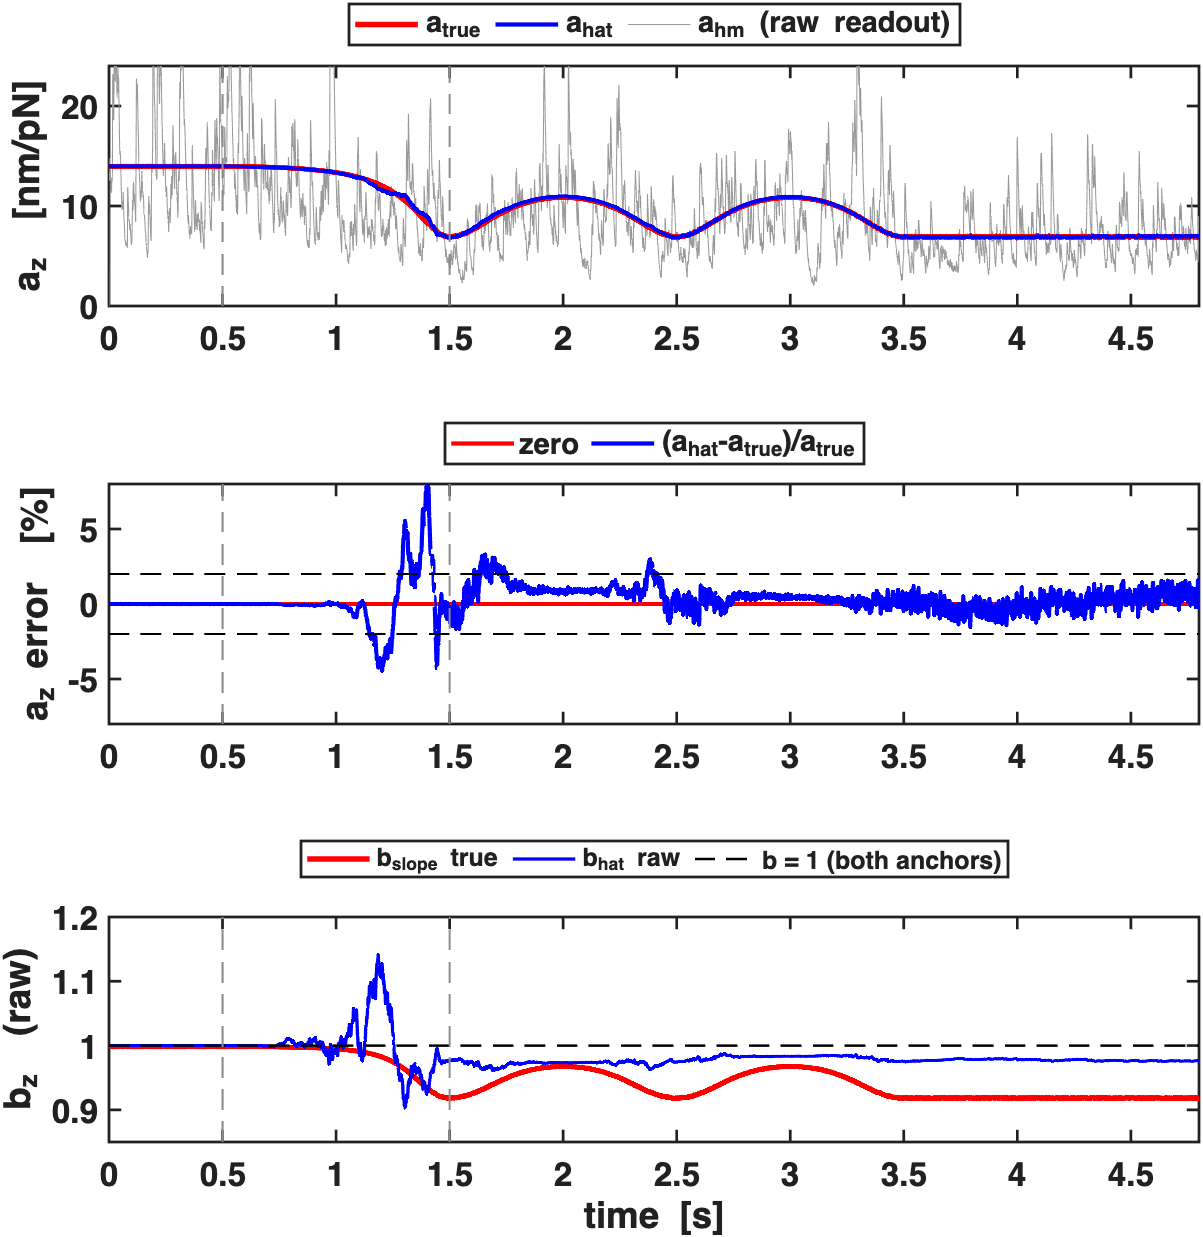
\includegraphics[width=\linewidth]{figures/expgain_5state_sim_diff.png}
\end{center}

\end{document}
